\newcommand{\rx}[1]{\texttt{"{\color{olive}#1}"}}
\newcommand{\match}[1]{{\color{blue}#1}}
\newcommand{\qtt}[1]{\texttt{"{#1}"}}

% =========================================================================== %

\begin{frame}[t,plain]
\titlepage
\end{frame}

% =========================================================================== %

\begin{frame}[fragile]{Five-Day Forecast}
%
\begin{center}
\begin{columns}
\column{.45\linewidth}
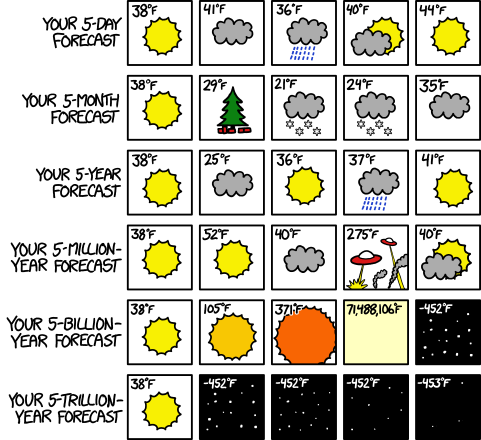
\includegraphics[width=\linewidth]{./gfx/00-xkcd-five_day_forecast}
%
\column{.45\linewidth}
\emph{You know what they say--if you don't like the weather here in the Solar System, just wait five billion years.}

\vspace{6pt}
Source: \url{https://xkcd.com/2259/}

\end{columns}
\end{center}
%
\end{frame}

% =========================================================================== %

\begin{frame}{About Me}
%
\begin{columns}[T]
\column{.45\linewidth}
\begin{itemize}
\item Former Student of UR
	\begin{itemize}
	\item 2015-2021: Physics
	\item 2020-2022: Computational Science
	\item Have been involved in UR IT courses since 2018
	\end{itemize}
\item Now: Software Development Engineer
\item Hobby enthusiast since childhood
	\begin{itemize}
	\item First programming language (BASIC) when I was 9 years old
	\item 25 years of semi-professional busying myself with computers
	\item I like sharing nerdy stuff in spite of my limited time
	\end{itemize}
\end{itemize}
%
\column{.55\linewidth}
\begin{itemize}
\item Human Languages
	\begin{itemize}
	\item German
	\item English
	\item French
	\end{itemize}
\item Computer Languages
	\begin{itemize}
	\item Python
	\item C, C++
	\item Java, Groovy
	\item BASIC (VisualBASIC, freeBASIC, QBASIC)
	\item \LaTeX
	\item (some Bash Shell Scripting, GnuPlot and Assembly; even less HTML, CSS, PowerShell, MS-DOS Batch and MySQL)
	\end{itemize}
\end{itemize}
\end{columns}
%
\end{frame}

% =========================================================================== %

\begin{frame}{Outlook}
%
%\small
\begin{columns}[T]
\column{.5\linewidth}
\begin{itemize}
\item What I've planned
	\begin{itemize}
	\footnotesize
	\item Guidelines for large projects (4 lectures) \\
		Maintainability considerations, SOLID Design Principles, Unit testing
	\item Internet architecture (3 lectures) \\
		OSI layers, TCP/IP, sockets, HTTP, HTML, XML, XSD
	\item String magic (3 lectures) \\
		RegExes, Template Code Generation, argparse and configparser
	\item Number Crunching (2 lectures) \\
		Symbolic Maths with SymPy, pandas data frames
	\item TBA (3 lectures) \\
		ideas: pickle, zipfile, hashes, string encodings, ...
	\end{itemize}
\end{itemize}
%
\column{.5\linewidth}
\begin{itemize}
\item Focus
	\begin{itemize}
	\footnotesize
	\item Broad concepts
	\item Examples from Python, ideas appicable beyond
	\end{itemize}
\item If you weren't here last semester
	\begin{itemize}
	\footnotesize
	\item \enquote{No dependencies}
	\item Sometimes: back-references with minimal explanation
	\item Watch videos in Mediathek if this sparked your interest
	\end{itemize}
\item But...
	\begin{itemize}
	\footnotesize
	\item My aim: fun and interesting content for you
	\item Your feedback will be heard! Tell me what you want to know!
	\item Unused lectures stay in GRIPS
	\end{itemize}
\end{itemize}
\end{columns}
%
\end{frame}

% =========================================================================== %

\begin{frame}{Don't Forget To Enroll in GRIPS}
%
\begin{columns}
\column{.3\linewidth}

\includegraphics[width=\linewidth]{./gfx/01-QR-GRIPS}
%
\column{.6\linewidth}
GRIPS \thus Physik \thus IT-Ausbildung, Elektronik \thus Python Booster Summer 2023/24

\vspace{6pt}
\url{https://elearning.uni-regensburg.de/course/view.php?id=39205}

\vspace{6pt}
Password: \emph{shrubbery2024}
\end{columns}
%
\end{frame}